%! Unidad 12 — Energía y trabajo: ejercicios resueltos, ejercicios finales y autoevaluación
%! Fuente: Fuentes/Fisica/Unidad 12 («Ejercicios resueltos», «Practica y calcula», «Piensa y resuelve») y Unidad 13 (captura 452:
%! «Autoevaluación» de este tema; la fuente no trae olimpiadas en este tema). Enunciados adaptados con datos cambiados (y más
%! realistas cuando los de la fuente no lo eran: trepar por una cuerda, potencia de un coche, disco giratorio); soluciones rehechas
%! con g = 9,8 m/s².
%! Dificultad: \(\star\) baja, \(\star\star\) media, \(\star\star\star\) alta.

\section{Ejercicios resueltos}\label{sec:ud12-resueltos}

\begin{example}
    \textbf{El carro de la compra.} Para llevar el carro de la compra, de \qty{22}{\kg}, desde la caja hasta la salida, a \qty{10}{\m},
    tiramos de él con una fuerza de \qty{120}{\newton} que forma \(30^\circ\) con la horizontal. El coeficiente de rozamiento con el
    suelo es \num{0.1}. Calcula el trabajo de cada fuerza y el trabajo total.

    \textbf{Solución.} \textbf{1. Fuerzas}: peso, normal, fuerza aplicada \(F\) (con componentes \(F_x = F\cos 30^\circ\) y
    \(F_y = F\sen 30^\circ\)) y rozamiento. Eje \(X\) en el sentido del movimiento.

    \textbf{2. La normal}: en el eje \(Y\) no hay movimiento: \(N + F_y - P = 0 \Rightarrow N = 22 \cdot \num{9.8} - 120\sen 30^\circ =
    \num{215.6} - 60 = \qty{155.6}{\newton}\); \(F_r = \mu\,N = \qty{15.6}{\newton}\).

    \textbf{3. Trabajo de cada fuerza}:
    \(W_F = 120 \cdot 10 \cdot \cos 30^\circ = \qty{1039}{\joule}\) (solo trabaja \(F_x\));
    \(W_P = W_N = 0\) (perpendiculares al desplazamiento);
    \(W_r = \num{15.6} \cdot 10 \cdot \cos 180^\circ = \qty{-156}{\joule}\).

    \textbf{4. Trabajo total}: \(W_{\text{total}} = 1039 + 0 + 0 - 156 = \qty{883}{\joule}\). Se comprueba que coincide con el trabajo
    de la resultante, que es horizontal: \(W = (F_x - F_r)\,\Delta x = (\num{103.9} - \num{15.6}) \cdot 10 = \qty{883}{\joule}\).
\end{example}

\begin{example}
    \textbf{Una montaña rusa con un looping.} La vagoneta de una montaña rusa, con sus ocupantes, tiene una masa de \qty{750}{\kg}.
    Sube hasta el punto A, a \qty{60}{\m} de altura, y desde allí se deja caer, prácticamente en reposo, hasta el punto más bajo, B,
    donde empieza un looping de \qty{12}{\m} de diámetro (figura~\ref{fig:ud12-looping}). Despreciando el rozamiento, calcula: a) la
    energía mecánica en A; b) la velocidad en B; c) la velocidad en lo alto del looping, C; d) la altura mínima de A para que la vagoneta
    complete el looping.

    \textbf{Solución.} \textbf{1.} Solo trabaja el peso (la normal es perpendicular a la vía): la energía mecánica se conserva. Tomamos
    como referencia de alturas el punto B.

    \textbf{2. a)} En A, \(v = 0\): \(E_m = m\,g\,h_A = 750 \cdot \num{9.8} \cdot 60 = \qty{4.41e5}{\joule}\).

    \textbf{3. b)} En B, \(h = 0\): \(\frac{1}{2}\,m\,v_B^2 = m\,g\,h_A \Rightarrow v_B = \sqrt{2 \cdot \num{9.8} \cdot 60} = \qty{34.3}{\m\per\s}\).

    \textbf{4. c)} En C, \(h_C = \qty{12}{\m}\): \(\frac{1}{2}\,m\,v_C^2 + m\,g\,h_C = m\,g\,h_A \Rightarrow v_C = \sqrt{2\,g\,(h_A - h_C)} =
    \sqrt{2 \cdot \num{9.8} \cdot 48} = \qty{30.7}{\m\per\s}\).

    \textbf{5. d)} En lo alto del looping, la fuerza centrípeta la hacen el peso y la normal (ambos hacia abajo): \(m\,g + N = m\,v_C^2/R\).
    La vagoneta sigue en contacto con la vía si \(N \geq 0\), es decir, si \(v_C^2 \geq g\,R\). Con la conservación de la energía:
    \[ 2\,g\,(h_A - 2R) \geq g\,R \Rightarrow h_A \geq \frac{5}{2}\,R = \num{2.5} \cdot 6 = \qty{15}{\m} \]
\end{example}

\begin{figure}[H]
    \centering
    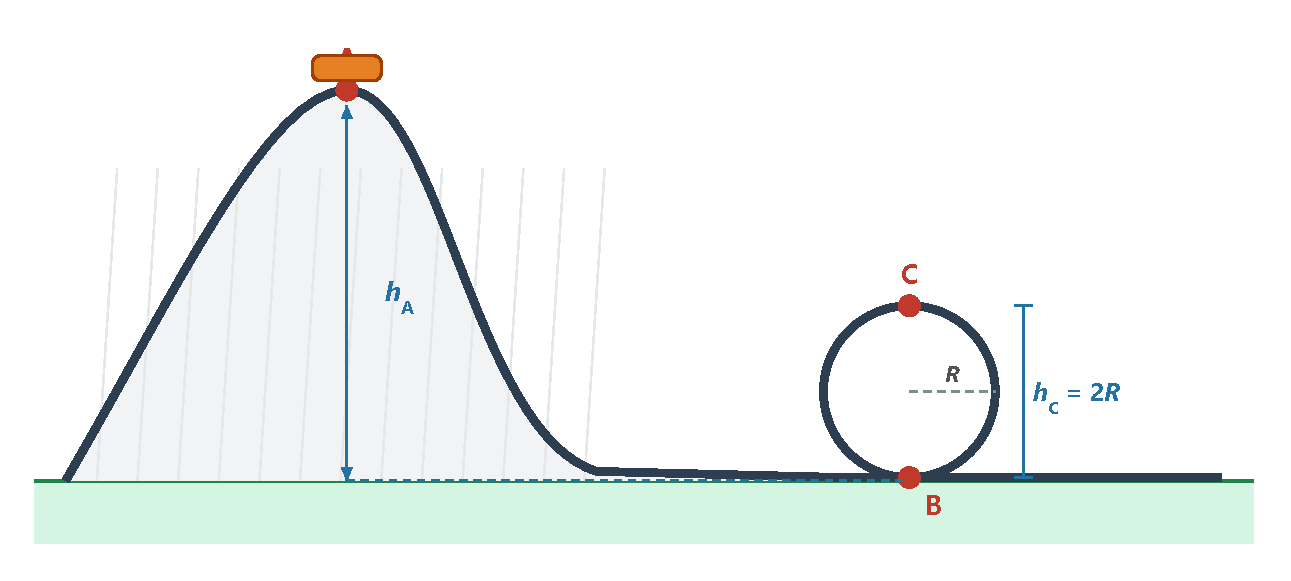
\includegraphics[width=0.75\textwidth]{images/UD12/montana_looping}
    \caption{Montaña rusa con un looping.}
    \label{fig:ud12-looping}
\end{figure}

\begin{example}
    \textbf{Subir y bajar por un plano.} Se lanza un bloque de \qty{3}{\kg} hacia arriba por un plano inclinado \(30^\circ\) con una
    velocidad de \qty{8}{\m\per\s}. El bloque se detiene, vuelve a bajar y llega al punto de partida con \qty{4}{\m\per\s}. Calcula: a) el
    trabajo total del rozamiento; b) la distancia que recorre al subir; c) el coeficiente de rozamiento.

    \textbf{Solución.} \textbf{a)} En el viaje de ida y vuelta, el peso no hace trabajo neto (es conservativo y el cuerpo vuelve al
    mismo punto) y la normal no trabaja. Solo trabaja el rozamiento:
    \(W_r = \Delta E_c = \frac{1}{2} \cdot 3 \cdot (4^2 - 8^2) = \qty{-72}{\joule}\).

    \textbf{b) y c)} Llamamos \(d\) a la distancia recorrida al subir; \(F_r = \mu\,m\,g\cos\alpha\) en los dos tramos.
    \[ \text{Subida: } \frac{1}{2}\,m\,v_0^2 = m\,g\,d\sen\alpha + F_r\,d \qquad \text{Bajada: } m\,g\,d\sen\alpha - F_r\,d = \frac{1}{2}\,m\,v_f^2 \]
    Sumando las dos ecuaciones (y dividiendo entre \(m\)):
    \[ \frac{1}{2}(v_0^2 + v_f^2) = 2\,g\,d\sen\alpha \Rightarrow d = \frac{64 + 16}{4 \cdot \num{9.8} \cdot \num{0.5}} = \qty{4.08}{\m} \]
    Restándolas:
    \[ \frac{1}{2}(v_0^2 - v_f^2) = 2\,\mu\,g\cos\alpha\,d \Rightarrow \mu = \frac{64 - 16}{4 \cdot \num{9.8} \cdot \cos 30^\circ \cdot \num{4.08}} = \num{0.35} \]
\end{example}

\begin{example}
    \textbf{Una lanzadera de coches.} Una pista de juguete tiene un muelle de constante \qty{500}{\newton\per\m}, un tramo horizontal de
    \qty{40}{\cm} y un plano inclinado \(30^\circ\). Se comprime el muelle \qty{6}{\cm} con un coche de \qty{200}{\g} y se suelta. El
    coeficiente de rozamiento es \num{0.15} en toda la pista. Calcula: a) la energía del muelle; b) la velocidad del coche al llegar al
    plano; c) la distancia que sube por el plano.

    \textbf{Solución.} \textbf{a)} \(E_p = \frac{1}{2} \cdot 500 \cdot \num{0.06}^2 = \qty{0.90}{\joule}\).

    \textbf{b)} En el tramo horizontal, \(W_r = -\mu\,m\,g\,d = -\num{0.15} \cdot \num{0.2} \cdot \num{9.8} \cdot \num{0.4} = \qty{-0.118}{\joule}\).
    Con \(W_{\text{no cons}} = \Delta E_m\): \(E_c = \num{0.90} - \num{0.118} = \qty{0.782}{\joule}\), y \(v = \sqrt{\dfrac{2 \cdot \num{0.782}}{\num{0.2}}} = \qty{2.80}{\m\per\s}\).

    \textbf{c)} En el plano, la energía cinética se invierte en subir y en vencer el rozamiento:
    \[ E_c = m\,g\,L\sen 30^\circ + \mu\,m\,g\cos 30^\circ\,L \Rightarrow L = \frac{\num{0.782}}{\num{0.2} \cdot \num{9.8} \cdot (\num{0.5} + \num{0.15} \cdot \num{0.866})}
    = \qty{0.63}{\m} \]
\end{example}

\begin{example}
    \textbf{Un montacargas.} El motor de un montacargas, con un rendimiento del \qty{80}{\percent}, sube una carga de \qty{500}{\kg} con
    una velocidad constante de \qty{1.5}{\m\per\s}. Calcula: a) la potencia útil; b) la potencia que consume el motor, en kW y en CV;
    c) la energía que consume para subir la carga \qty{30}{\m}, en julios y en kWh.

    \textbf{Solución.} \textbf{a)} A velocidad constante, la fuerza del cable iguala al peso: \(P_{\text{útil}} = F\,v = m\,g\,v =
    500 \cdot \num{9.8} \cdot \num{1.5} = \qty{7350}{\watt}\).

    \textbf{b)} \(P_{\text{consumida}} = \dfrac{P_{\text{útil}}}{\eta} \cdot 100 = \dfrac{7350}{80} \cdot 100 = \qty{9188}{\watt} =
    \qty{9.19}{\kilo\watt}\), es decir, \(\dfrac{9188}{735} = \num{12.5}\)~CV.

    \textbf{c)} Tarda \(t = 30/\num{1.5} = \qty{20}{\s}\): \(E = 9188 \cdot 20 = \qty{1.84e5}{\joule} = \qty{0.051}{\kilo\watt\hour}\).
\end{example}

%========================================================================================
\section{Ejercicios de aplicación}\label{sec:ud12-aplicacion}
%========================================================================================

\subsection{La energía: concepto y tipos}

\begin{exercise}
    \(\star\) ¿Qué es la energía? ¿De dónde procede la que usamos en la Tierra?
    \begin{solu}
        \textcolor{red}{Es la capacidad de los sistemas para producir cambios}. Casi toda procede, directa o indirectamente, del
        \textcolor{red}{Sol} (combustibles fósiles, viento, ciclo del agua, biomasa); el resto, de la \textcolor{red}{energía nuclear}
        de los átomos y del \textcolor{red}{calor interno de la Tierra}.
    \end{solu}
\end{exercise}

\begin{exercise}
    \(\star\) La energía nuclear y la química están relacionadas con los átomos. ¿En qué se diferencian?
    \begin{solu}
        La \textcolor{red}{química} está asociada a los \textcolor{red}{enlaces entre átomos} (los electrones) y se libera en las
        reacciones químicas; la \textcolor{red}{nuclear}, a las fuerzas que mantienen unido el \textcolor{red}{núcleo}, y se libera en la
        fisión y en la fusión, en cantidades millones de veces mayores.
    \end{solu}
\end{exercise}

\begin{exercise}
    \(\star\) Cuando una pila deja de funcionar, decimos que «se ha gastado la energía». Si la energía se conserva, ¿es correcta esta
    afirmación?
    \begin{solu}
        \textcolor{red}{No del todo}: la energía química de la pila no ha desaparecido, se ha transformado en otras formas (eléctrica,
        luminosa, térmica\dots) que ya no podemos aprovechar. La energía se ha \textcolor{red}{degradado}.
    \end{solu}
\end{exercise}

\begin{exercise}
    \(\star\) Indica qué forma de energía interviene en cada caso: a) un muelle comprimido; b) una pila de combustible de hidrógeno;
    c) una bombona de butano; d) las señales de los satélites GPS; e) las aspas de un aerogenerador; f) una noria en movimiento;
    g) la radioterapia; h) un secador de pelo; i) un arco a punto de disparar; j) los protones del acelerador del CERN.
    \begin{solu}
        a) \textcolor{red}{Potencial elástica}. b) \textcolor{red}{Química} (que da eléctrica). c) \textcolor{red}{Química}.
        d) \textcolor{red}{Electromagnética}. e) \textcolor{red}{Cinética}. f) \textcolor{red}{Mecánica} (cinética y potencial).
        g) \textcolor{red}{Electromagnética} o \textcolor{red}{nuclear}. h) \textcolor{red}{Eléctrica}, que se transforma en térmica y
        cinética. i) \textcolor{red}{Potencial elástica}. j) \textcolor{red}{Cinética}.
    \end{solu}
\end{exercise}

\begin{exercise}
    \(\star\) Define con tus palabras qué son las fuentes de energía renovables y no renovables, y clasifica estas: a) combustibles
    fósiles; b) biomasa; c) sol, agua y viento; d) uranio; e) geotérmica.
    \begin{solu}
        \textcolor{red}{Renovables}: b), c) y e). \textcolor{red}{No renovables}: a) y d).
    \end{solu}
\end{exercise}

\begin{exercise}
    \(\star\star\) Busca información sobre las aportaciones de Leibniz, Mayer y Joule al concepto de energía y escribe un breve informe.
    \begin{solu}
        \textcolor{red}{Respuesta abierta}. Leibniz: la \textit{vis viva} (\(m\,v^2\)) que se conserva en los choques; Mayer: primera
        formulación del principio de conservación de la energía; Joule: equivalente mecánico del calor.
    \end{solu}
\end{exercise}

\subsection{El trabajo}

\begin{exercise}
    \(\star\) ¿Es lo mismo trabajo que esfuerzo? Indica si hay trabajo en estas actividades: a) poner un plato en la mesa; b) empujar un
    armario que no se mueve; c) llevar la compra a casa por la calle, sin subir ni bajar; d) hacer una plancha de yoga sin moverse.
    \begin{solu}
        \textcolor{red}{No}. a) \textcolor{red}{Sí} (se levanta el plato). b) \textcolor{red}{No}. c) La fuerza vertical que sostiene la
        bolsa \textcolor{red}{no trabaja} (es perpendicular al desplazamiento). d) \textcolor{red}{No}.
    \end{solu}
\end{exercise}

\begin{exercise}
    \(\star\star\) La fuerza que actúa sobre un cuerpo, paralela al desplazamiento, crece uniformemente desde 0 hasta \qty{40}{\newton}
    en los primeros \qty{2}{\m} y se mantiene en \qty{40}{\newton} hasta \(x = \qty{5}{\m}\). Dibuja la gráfica \(F\)-\(x\) y calcula el
    trabajo.
    \begin{solu}
        Área de un triángulo más un rectángulo: \(W = \frac{1}{2} \cdot 2 \cdot 40 + 3 \cdot 40 = \textcolor{red}{\qty{160}{\joule}}\).
    \end{solu}
\end{exercise}

\begin{exercise}
    \(\star\star\) ¿Hay alguna fuerza que realice trabajo sobre un cuerpo con movimiento circular uniforme? Justifícalo.
    \begin{solu}
        \textcolor{red}{No}: la fuerza neta es centrípeta, perpendicular a la velocidad, y su trabajo es nulo; de hecho, la energía
        cinética no cambia.
    \end{solu}
\end{exercise}

\begin{exercise}
    \(\star\star\) ¿El trabajo de la fuerza de rozamiento es siempre negativo?
    \begin{solu}
        \textcolor{red}{No siempre}. El rozamiento cinético sobre un cuerpo que desliza sobre una superficie fija sí realiza trabajo
        negativo, pero el rozamiento estático puede hacer \textcolor{red}{trabajo positivo}: el que la plataforma de un camión que acelera
        hace sobre una caja que no desliza, o el de una cinta transportadora sobre las maletas.
    \end{solu}
\end{exercise}

\begin{exercise}
    \(\star\star\) Calcula el trabajo en estas situaciones: a) la fuerza que hacemos para sostener sobre los hombros, sin movernos, a una
    persona de \qty{60}{\kg}; b) una fuerza horizontal de \qty{15}{\newton} que desplaza \qty{1.2}{\m} un cuerpo de \qty{30}{\kg} por un
    suelo sin rozamiento; c) la fuerza gravitatoria de la Tierra sobre la Luna, supuesta su órbita circular.
    \begin{solu}
        a) \(\textcolor{red}{0}\). b) \(\textcolor{red}{\qty{18}{\joule}}\). c) \(\textcolor{red}{0}\).
    \end{solu}
\end{exercise}

\begin{exercise}
    \(\star\) Una grúa portuaria levanta un contenedor de \qty{12}{t} a \qty{15}{\m} de altura. ¿Qué trabajo realiza?
    \begin{solu}
        \(W = m\,g\,h = 12\,000 \cdot \num{9.8} \cdot 15 = \textcolor{red}{\qty{1.76e6}{\joule}}\).
    \end{solu}
\end{exercise}

\begin{exercise}
    \(\star\star\) Sobre un cuerpo de \qty{15}{\kg}, que se desplaza \qty{50}{\m} por un plano horizontal, actúa una fuerza de
    \qty{80}{\newton}. Calcula su trabajo si: a) forma \(40^\circ\) con la horizontal; b) es perpendicular al desplazamiento; c) tiene la
    dirección y el sentido del movimiento; d) forma \(135^\circ\) con el desplazamiento.
    \begin{solu}
        a) \(\textcolor{red}{\qty{3.06e3}{\joule}}\). b) \(\textcolor{red}{0}\). c) \(\textcolor{red}{\qty{4.00e3}{\joule}}\).
        d) \(\textcolor{red}{\qty{-2.83e3}{\joule}}\).
    \end{solu}
\end{exercise}

\begin{exercise}
    \(\star\star\) Un cuerpo de \qty{25}{\kg} baja \qty{2}{\m} deslizando por un plano inclinado \(30^\circ\), con un coeficiente de
    rozamiento de \num{0.25}. ¿Qué trabajo total recibe?
    \begin{solu}
        \(W_P = 25 \cdot \num{9.8} \cdot 2 \cdot \sen 30^\circ = \qty{245}{\joule}\); \(W_r = -\num{0.25} \cdot 25 \cdot \num{9.8} \cdot \cos 30^\circ
        \cdot 2 = \qty{-106}{\joule}\); \(W_{\text{total}} = \textcolor{red}{\qty{139}{\joule}}\).
    \end{solu}
\end{exercise}

\begin{exercise}
    \(\star\star\) Una bomba sube agua a un depósito de \qty{300}{\liter} situado en la azotea de un edificio de \qty{60}{\m} de altura.
    ¿Qué trabajo realiza la bomba como mínimo?
    \begin{solu}
        \(W = 300 \cdot \num{9.8} \cdot 60 = \textcolor{red}{\qty{1.76e5}{\joule}}\).
    \end{solu}
\end{exercise}

\subsection{La energía cinética}

\begin{exercise}
    \(\star\) ¿La energía cinética puede ser negativa? ¿Y su variación?
    \begin{solu}
        La energía cinética \textcolor{red}{nunca es negativa}, porque \(m\) y \(v^2\) son positivos. Su \textcolor{red}{variación sí
        puede ser negativa}, cuando el cuerpo frena.
    \end{solu}
\end{exercise}

\begin{exercise}
    \(\star\) ¿De qué depende la energía cinética de un cuerpo? ¿Cómo cambia si se duplica su masa? ¿Y si se duplica su velocidad?
    \begin{solu}
        De la \textcolor{red}{masa y de la velocidad}. Si se duplica la masa, \textcolor{red}{se duplica}; si se duplica la velocidad,
        \textcolor{red}{se multiplica por cuatro}.
    \end{solu}
\end{exercise}

\begin{exercise}
    \(\star\) Explica con tus palabras el teorema de las fuerzas vivas y pon un ejemplo.
    \begin{solu}
        \textcolor{red}{El trabajo de todas las fuerzas que actúan sobre un cuerpo es igual a la variación de su energía cinética}. Por
        ejemplo, al frenar una bici, el trabajo negativo del rozamiento de los frenos disminuye su energía cinética.
    \end{solu}
\end{exercise}

\begin{exercise}
    \(\star\star\) ¿Qué tiene más energía cinética, una moto de \qty{180}{\kg} a \qty{120}{\km\per\hour} o un coche eléctrico de
    \qty{1700}{\kg} a \qty{50}{\km\per\hour}?
    \begin{solu}
        Moto: \(\textcolor{red}{\qty{1.00e5}{\joule}}\); coche: \(\textcolor{red}{\qty{1.64e5}{\joule}}\). \textcolor{red}{El coche}.
    \end{solu}
\end{exercise}

\begin{exercise}
    \(\star\star\) Calcula el trabajo que realiza una ciclista, que con su bicicleta tiene una masa de \qty{85}{\kg}, cuando su velocidad
    aumenta de \qty{30}{\km\per\hour} a \qty{50}{\km\per\hour}. Desprecia el rozamiento.
    \begin{solu}
        \(W = \frac{1}{2} \cdot 85 \cdot (\num{13.89}^2 - \num{8.33}^2) = \textcolor{red}{\qty{5.25e3}{\joule}}\).
    \end{solu}
\end{exercise}

\begin{exercise}
    \(\star\star\) Una roca de \qty{900}{\kg} rueda ladera abajo y llega al pie de la colina con una energía cinética de
    \qty{120000}{\joule}. ¿Con qué velocidad llega?
    \begin{solu}
        \(v = \sqrt{\dfrac{2 \cdot 120\,000}{900}} = \textcolor{red}{\qty{16.3}{\m\per\s}}\).
    \end{solu}
\end{exercise}

\begin{exercise}
    \(\star\star\) Lanzamos una canica de \qty{8}{\g} por el suelo a \qty{2.5}{\m\per\s} y se detiene a los \qty{4}{\m}. ¿Qué fuerza de
    rozamiento ha actuado sobre ella?
    \begin{solu}
        \(F_r\,d = \frac{1}{2}\,m\,v^2 \Rightarrow F_r = \dfrac{\num{0.025}}{4} = \textcolor{red}{\qty{6.3e-3}{\newton}}\).
    \end{solu}
\end{exercise}

\begin{exercise}
    \(\star\star\) Un tren de alta velocidad de \qty{400}{t} circula a \qty{200}{\km\per\hour}. ¿Qué velocidad alcanzará si el trabajo
    neto de las fuerzas que actúan sobre él es de \qty{8.0e8}{\joule}?
    \begin{solu}
        \(E_{c,i} = \qty{6.17e8}{\joule}\); \(E_{c,f} = \qty{1.42e9}{\joule}\); \(v = \textcolor{red}{\qty{84.2}{\m\per\s}} = \qty{303}{\km\per\hour}\).
    \end{solu}
\end{exercise}

\subsection{La energía potencial}

\begin{exercise}
    \(\star\) Un cuerpo está en el fondo de un pozo. ¿Tiene energía potencial gravitatoria?
    \begin{solu}
        Depende del \textcolor{red}{nivel de referencia}. Si lo tomamos en el suelo, su energía potencial es
        \textcolor{red}{negativa}; si lo tomamos en el fondo del pozo, es nula.
    \end{solu}
\end{exercise}

\begin{exercise}
    \(\star\star\) Un cuerpo lleva una velocidad de \qty{72}{\km\per\hour}. ¿A qué altura debería estar para que su energía potencial
    fuera igual a esa energía cinética?
    \begin{solu}
        \(m\,g\,h = \frac{1}{2}\,m\,v^2 \Rightarrow h = \dfrac{20^2}{2 \cdot \num{9.8}} = \textcolor{red}{\qty{20.4}{\m}}\).
    \end{solu}
\end{exercise}

\begin{exercise}
    \(\star\) Si un muelle no está ni comprimido ni estirado, ¿tiene energía potencial elástica?
    \begin{solu}
        \textcolor{red}{No}: \(x = 0\), así que \(E_p = 0\).
    \end{solu}
\end{exercise}

\begin{exercise}
    \(\star\star\) Cuenta la leyenda que Newton pensó en la gravitación al ver caer una manzana. Si la manzana tenía \qty{120}{\g} y
    estaba a \qty{4}{\m} de altura, ¿qué energía potencial tenía?
    \begin{solu}
        \(E_p = \num{0.12} \cdot \num{9.8} \cdot 4 = \textcolor{red}{\qty{4.70}{\joule}}\).
    \end{solu}
\end{exercise}

\begin{exercise}
    \(\star\star\) Dos paracaidistas, con una masa conjunta de \qty{170}{\kg}, saltan en tándem desde lo alto del Burj Khalifa
    (\qty{828}{\m}). Suponiendo que no hubiera rozamiento con el aire, calcula: a) su energía potencial inicial; b) su energía potencial a
    \qty{414}{\m} de altura; c) su velocidad y su energía cinética a esa altura; d) la suma de b) y c). e) ¿Por qué en la realidad la
    velocidad es mucho menor?
    \begin{solu}
        a) \(\textcolor{red}{\qty{1.38e6}{\joule}}\). b) \(\textcolor{red}{\qty{6.90e5}{\joule}}\). c) \(\textcolor{red}{\qty{90.1}{\m\per\s}}\);
        \(\textcolor{red}{\qty{6.90e5}{\joule}}\). d) \(\textcolor{red}{\qty{1.38e6}{\joule}}\): la energía mecánica se conserva.
        e) \textcolor{red}{Por la resistencia del aire}, que limita la velocidad de caída a unos \qty{55}{\m\per\s}.
    \end{solu}
\end{exercise}

\begin{exercise}
    \(\star\star\) Un deportista de \qty{75}{\kg} hace 8 dominadas, subiendo cada vez \qty{0.6}{\m}. Calcula: a) el trabajo que hace
    contra su peso; b) su energía potencial en lo alto de una dominada, respecto a la posición inicial; c) su energía cinética cuando
    corre a \qty{2}{\m\per\s}.
    \begin{solu}
        a) \(W = 8 \cdot 75 \cdot \num{9.8} \cdot \num{0.6} = \textcolor{red}{\qty{3.53e3}{\joule}}\). b) \(\textcolor{red}{\qty{441}{\joule}}\).
        c) \(\textcolor{red}{\qty{150}{\joule}}\).
    \end{solu}
\end{exercise}

\begin{exercise}
    \(\star\star\) Al colgar una masa de \qty{2}{\kg} de un muelle, se estira \qty{5}{\cm}. ¿Cuál es su constante elástica? ¿Qué energía
    potencial elástica almacena?
    \begin{solu}
        \(k = \textcolor{red}{\qty{392}{\newton\per\m}}\); \(E_p = \textcolor{red}{\qty{0.49}{\joule}}\).
    \end{solu}
\end{exercise}

\begin{exercise}
    \(\star\star\) Un resorte de constante \qty{200}{\newton\per\m} mide \qty{40}{\cm}. ¿Qué trabajo hay que hacer para comprimirlo hasta
    que mida \qty{28}{\cm}?
    \begin{solu}
        \(W = \frac{1}{2} \cdot 200 \cdot \num{0.12}^2 = \textcolor{red}{\qty{1.44}{\joule}}\).
    \end{solu}
\end{exercise}

\begin{exercise}
    \(\star\star\) Un halcón peregrino de \qty{1}{\kg} vuela a \qty{60}{\m} de altura y se lanza en picado, desde el reposo, a por una
    presa. Despreciando el rozamiento, calcula: a) su energía potencial inicial; b) su energía potencial a \qty{20}{\m} del suelo; c) su
    velocidad y su energía cinética a esa altura.
    \begin{solu}
        a) \(\textcolor{red}{\qty{588}{\joule}}\). b) \(\textcolor{red}{\qty{196}{\joule}}\). c) \(E_c = \textcolor{red}{\qty{392}{\joule}}\);
        \(v = \textcolor{red}{\qty{28.0}{\m\per\s}}\).
    \end{solu}
\end{exercise}

\subsection{La energía mecánica}

\begin{exercise}
    \(\star\star\) Explica con tus palabras qué es la energía mecánica y en qué condiciones se conserva.
    \begin{solu}
        \textcolor{red}{Es la suma de la energía cinética y la potencial}. \textcolor{red}{Se conserva si solo realizan trabajo fuerzas
        conservativas} (no hay rozamiento ni otras fuerzas que trabajen).
    \end{solu}
\end{exercise}

\begin{exercise}
    \(\star\star\) Un avión de \qty{400}{t} vuela a \qty{900}{\km\per\hour} a \qty{11}{\km} de altura. ¿Cuál es su energía mecánica
    respecto al suelo?
    \begin{solu}
        \(E_c = \qty{1.25e10}{\joule}\); \(E_p = \qty{4.31e10}{\joule}\); \(E_m = \textcolor{red}{\qty{5.56e10}{\joule}}\).
    \end{solu}
\end{exercise}

\begin{exercise}
    \(\star\star\) A una escaladora se le cae la mochila, de \qty{2}{\kg}, desde \qty{25}{\m} de altura. Despreciando el rozamiento,
    calcula: a) la energía potencial de la mochila cuando ha caído \qty{10}{\m}; b) su velocidad a \qty{4}{\m} del suelo.
    \begin{solu}
        a) \(E_p = 2 \cdot \num{9.8} \cdot 15 = \textcolor{red}{\qty{294}{\joule}}\). b) \(v = \sqrt{2 \cdot \num{9.8} \cdot 21} =
        \textcolor{red}{\qty{20.3}{\m\per\s}}\).
    \end{solu}
\end{exercise}

\begin{exercise}
    \(\star\star\) Una gimnasta de trampolín sale hacia arriba con \qty{10}{\m\per\s}. Calcula: a) la altura máxima que alcanza sobre
    el trampolín; b) su velocidad a \qty{3}{\m} de altura; c) a qué altura su velocidad es de \qty{6}{\m\per\s}.
    \begin{solu}
        a) \(h = \dfrac{v^2}{2\,g} = \textcolor{red}{\qty{5.10}{\m}}\). b) \(v = \sqrt{100 - 2 \cdot \num{9.8} \cdot 3} = \textcolor{red}{\qty{6.42}{\m\per\s}}\).
        c) \(h = \dfrac{100 - 36}{2 \cdot \num{9.8}} = \textcolor{red}{\qty{3.27}{\m}}\).
    \end{solu}
\end{exercise}

\begin{exercise}
    \(\star\star\) Un coche teledirigido de \qty{1.2}{\kg} se queda sin batería cuando va a \qty{5}{\m\per\s}, justo al empezar a subir
    una rampa de \(25^\circ\). Si el coeficiente de rozamiento es \num{0.2}, ¿a qué altura se detiene?
    \begin{solu}
        \(\frac{1}{2}\,m\,v^2 = m\,g\,d\,(\sen 25^\circ + \mu\cos 25^\circ) \Rightarrow d = \qty{2.11}{\m}\);
        \(h = d\sen 25^\circ = \textcolor{red}{\qty{0.89}{\m}}\).
    \end{solu}
\end{exercise}

\begin{exercise}
    \(\star\star\) La vagoneta de una montaña rusa, con sus ocupantes, tiene \qty{800}{\kg}. Parte del reposo desde lo alto de la
    primera subida, a \qty{70}{\m}, y baja hasta lo alto de la segunda, a \qty{40}{\m}. Sin rozamiento: a) ¿con qué velocidad pasa por
    la segunda cima? b) ¿Qué trabajo ha hecho el motor para subirla hasta los \qty{70}{\m}?
    \begin{solu}
        a) \(v = \sqrt{2 \cdot \num{9.8} \cdot 30} = \textcolor{red}{\qty{24.2}{\m\per\s}}\). b) \(W = m\,g\,h = \textcolor{red}{\qty{5.49e5}{\joule}}\).
    \end{solu}
\end{exercise}

\begin{exercise}
    \(\star\star\) Una bola de \qty{200}{\g} cuelga de un hilo de \qty{1}{\m}. Se separa hasta que el hilo forma \(60^\circ\) con la
    vertical y se suelta. Calcula su velocidad y la tensión del hilo en el punto más bajo.
    \begin{solu}
        Baja \(h = 1 - \cos 60^\circ = \qty{0.5}{\m}\): \(v = \sqrt{2\,g\,h} = \textcolor{red}{\qty{3.13}{\m\per\s}}\).
        \(T - m\,g = m\,v^2/L \Rightarrow T = \num{1.96} + \num{1.96} = \textcolor{red}{\qty{3.92}{\newton}}\).
    \end{solu}
\end{exercise}

\subsection{Potencia y rendimiento}

\begin{exercise}
    \(\star\) Explica con tus palabras el concepto de potencia y pon ejemplos.
    \begin{solu}
        \textcolor{red}{Es la rapidez con que se realiza un trabajo o se transfiere energía}. Por ejemplo, un ascensor y una persona
        hacen el mismo trabajo al subir una caja, pero el ascensor lo hace en menos tiempo: tiene más potencia.
    \end{solu}
\end{exercise}

\begin{exercise}
    \(\star\star\) ¿Qué potencia desarrolla una grúa que eleva un coche de \qty{1200}{\kg} a \qty{4}{\m} de altura en \qty{12}{\s}?
    Exprésala en kW y en CV.
    \begin{solu}
        \(P = \dfrac{1200 \cdot \num{9.8} \cdot 4}{12} = \textcolor{red}{\qty{3.92}{\kilo\watt}}\) = \textcolor{red}{\num{5.3}~CV}.
    \end{solu}
\end{exercise}

\begin{exercise}
    \(\star\star\) Un coche de carreras de \qty{800}{\kg} pasa de 0 a \qty{100}{\km\per\hour} en \qty{2.6}{\s}. Si el \qty{25}{\percent}
    de la energía que da el motor se pierde por rozamiento, calcula: a) la energía cinética final; b) la potencia media del motor.
    \begin{solu}
        a) \(E_c = \frac{1}{2} \cdot 800 \cdot \num{27.8}^2 = \textcolor{red}{\qty{3.09e5}{\joule}}\). b) El motor aporta
        \(\dfrac{\num{3.09e5}}{\num{0.75}} = \qty{4.12e5}{\joule}\): \(P = \textcolor{red}{\qty{158}{\kilo\watt}}\).
    \end{solu}
\end{exercise}

\begin{exercise}
    \(\star\star\) En una central hidroeléctrica caen \qty{40}{\m\cubed} de agua desde \qty{50}{\m} de altura. Si se aprovecha el
    \qty{85}{\percent} de la energía, ¿cuántas bombillas LED de \qty{10}{\watt} podrían estar encendidas durante una hora?
    \begin{solu}
        \(E = \num{4e4} \cdot \num{9.8} \cdot 50 \cdot \num{0.85} = \qty{1.67e7}{\joule}\); \(n = \dfrac{\num{1.67e7}}{10 \cdot 3600} =
        \textcolor{red}{462~bombillas}\).
    \end{solu}
\end{exercise}

\begin{exercise}
    \(\star\star\) Investiga cómo es la etiqueta energética de los electrodomésticos que se usa en la Unión Europea desde 2021 y qué
    cambió respecto a la anterior.
    \begin{solu}
        \textcolor{red}{Respuesta abierta}: la nueva escala va de la A a la G (desaparecen las clases A+, A++ y A+++), es más exigente,
        indica el consumo en kWh y lleva un código QR con información del producto.
    \end{solu}
\end{exercise}

\begin{exercise}
    \(\star\star\) El motor de una grúa, con sus engranajes, tiene un rendimiento del \qty{60}{\percent}. ¿Qué potencia consume para
    subir unas vigas de \qty{500}{\kg} a \qty{18}{\m} de altura en \qty{1.5}{\minute}?
    \begin{solu}
        \(P_{\text{útil}} = \dfrac{500 \cdot \num{9.8} \cdot 18}{90} = \qty{980}{\watt}\); \(P = \dfrac{980}{\num{0.6}} = \textcolor{red}{\qty{1.63}{\kilo\watt}}\).
    \end{solu}
\end{exercise}

\begin{exercise}
    \(\star\star\) En la azotea de un edificio de \qty{30}{\m} hay un depósito de \qty{250}{\liter}. El motor que sube el agua tiene una
    potencia de \qty{400}{\watt} y tarda \qty{4}{\minute} en llenarlo. ¿Cuál es su rendimiento?
    \begin{solu}
        \(W_{\text{útil}} = 250 \cdot \num{9.8} \cdot 30 = \qty{73500}{\joule}\); \(E = 400 \cdot 240 = \qty{96000}{\joule}\);
        \(\eta = \textcolor{red}{\qty{77}{\percent}}\).
    \end{solu}
\end{exercise}

\begin{exercise}
    \(\star\star\) El frigorífico es el electrodoméstico que más consume en una casa, alrededor del \qty{14}{\percent} del total. La
    etiqueta de uno indica un consumo de \qty{150}{\kilo\watt\hour} al año. Calcula su consumo diario en julios y estima el consumo
    anual del hogar.
    \begin{solu}
        \(\dfrac{150}{365} = \qty{0.411}{\kilo\watt\hour}\) = \(\textcolor{red}{\qty{1.48e6}{\joule}}\) al día; hogar:
        \(\dfrac{150}{\num{0.14}} = \textcolor{red}{\qty{1071}{\kilo\watt\hour}}\) al año.
    \end{solu}
\end{exercise}

%========================================================================================
\section{Ejercicios de ampliación}\label{sec:ud12-ampliacion}
%========================================================================================

\begin{exercise}
    \(\star\star\star\) Una jugadora de voleibol salta para bloquear un remate. ¿De dónde sale la energía que la eleva por encima de la
    red? ¿Qué fuerza la impulsa hacia arriba? ¿Realiza trabajo esa fuerza?
    \begin{solu}
        La energía sale de la \textcolor{red}{energía química de sus músculos}. La fuerza que la impulsa es la
        \textcolor{red}{normal del suelo} (reacción a la fuerza con que sus piernas empujan el suelo), pero
        \textcolor{red}{no realiza trabajo}, porque su punto de aplicación (los pies sobre el suelo) no se desplaza: el trabajo lo
        hacen fuerzas internas de su cuerpo.
    \end{solu}
\end{exercise}

\begin{exercise}
    \(\star\star\star\) Un helicóptero rescata a un senderista de \qty{80}{\kg} elevándolo con un cable que tira de él con una fuerza
    constante de \qty{820}{\newton}. Si parte del reposo, ¿qué velocidad tiene tras subir los \qty{15}{\m} de cable?
    \begin{solu}
        \(W_{\text{total}} = (820 - 80 \cdot \num{9.8}) \cdot 15 = \qty{540}{\joule} = \frac{1}{2}\,m\,v^2 \Rightarrow v = \textcolor{red}{\qty{3.67}{\m\per\s}}\).
    \end{solu}
\end{exercise}

\begin{exercise}
    \(\star\star\star\) El disco de una amoladora, de \qty{12.5}{\cm} de diámetro, gira a \qty{10000}{rpm}. La pieza que se corta ejerce
    sobre el borde del disco una fuerza de rozamiento de \qty{6}{\newton}. ¿Qué potencia debe dar el motor para mantener el giro?
    \begin{solu}
        \(v = \omega\,r = \dfrac{10\,000 \cdot 2\pi}{60} \cdot \num{0.0625} = \qty{65.4}{\m\per\s}\); \(P = F\,v = \textcolor{red}{\qty{393}{\watt}}\).
    \end{solu}
\end{exercise}

\begin{exercise}
    \(\star\star\star\) Un muelle de constante \qty{800}{\newton\per\m}, comprimido \qty{10}{\cm}, lanza un bloque de \qty{500}{\g} por
    una superficie horizontal con un coeficiente de rozamiento de \num{0.2}. ¿Qué distancia recorre el bloque hasta pararse?
    \begin{solu}
        \(\frac{1}{2}\,k\,x^2 = \mu\,m\,g\,d \Rightarrow d = \dfrac{4}{\num{0.2} \cdot \num{0.5} \cdot \num{9.8}} = \textcolor{red}{\qty{4.08}{\m}}\).
    \end{solu}
\end{exercise}

\begin{exercise}
    \(\star\star\star\) En la carrera de camellos de una feria se lanzan bolas hacia arriba por una rampa inclinada \(35^\circ\) para que
    entren en unos agujeros. Una bola lanzada a \qty{7}{\m\per\s} llega justo al último agujero, que está a \qty{2}{\m} de altura. ¿Cuál
    es el coeficiente de rozamiento?
    \begin{solu}
        \(\frac{1}{2}\,v_0^2 = g\,h + \mu\,g\cos 35^\circ \dfrac{h}{\sen 35^\circ} \Rightarrow \num{24.5} = \num{19.6} + \num{27.99}\,\mu
        \Rightarrow \mu = \textcolor{red}{\num{0.18}}\).
    \end{solu}
\end{exercise}

\begin{exercise}
    \(\star\star\star\) Un camión de juguete de \qty{1}{\kg} se suelta desde lo alto de un plano inclinado \(30^\circ\) de \qty{1}{\m}
    de longitud; luego sigue por una pista horizontal y se para tras recorrer \qty{2}{\m}. El coeficiente de rozamiento es el mismo en todo
    el recorrido. Calcula: a) el coeficiente de rozamiento; b) la energía disipada en cada tramo; c) la velocidad al final del plano.
    \begin{solu}
        a) \(m\,g\,L\sen 30^\circ = \mu\,m\,g\,(L\cos 30^\circ + d) \Rightarrow \mu = \dfrac{\num{0.5}}{\num{0.866} + 2} = \textcolor{red}{\num{0.17}}\).
        b) Plano: \(\textcolor{red}{\qty{1.48}{\joule}}\); horizontal: \(\textcolor{red}{\qty{3.42}{\joule}}\) (en total, los
        \qty{4.9}{\joule} de energía potencial inicial). c) \(E_c = \num{4.9} - \num{1.48} = \qty{3.42}{\joule}\); \(v = \textcolor{red}{\qty{2.62}{\m\per\s}}\).
    \end{solu}
\end{exercise}

\begin{exercise}
    \(\star\star\star\) Un cuerpo de \qty{2}{\kg} empieza a bajar con \qty{3}{\m\per\s} por un plano inclinado \(20^\circ\) y de
    \qty{4}{\m} de longitud, sin rozamiento. Al final del plano choca con un muelle de constante \qty{500}{\newton\per\m}. a) ¿Con qué
    velocidad llega al final del plano? b) ¿Cuánto comprime el muelle?
    \begin{solu}
        a) \(v = \sqrt{9 + 2 \cdot \num{9.8} \cdot 4\sen 20^\circ} = \textcolor{red}{\qty{5.98}{\m\per\s}}\).
        b) \(\frac{1}{2}\,m\,v^2 = \frac{1}{2}\,k\,x^2 \Rightarrow x = v\sqrt{m/k} = \textcolor{red}{\qty{0.38}{\m}}\) (suponiendo el
        muelle en la parte horizontal).
    \end{solu}
\end{exercise}

\begin{exercise}
    \(\star\star\star\) Un coche de \qty{1300}{\kg} sube a \qty{90}{\km\per\hour} constantes una carretera con una pendiente del
    \qty{8}{\percent} (sube \qty{8}{\m} por cada \qty{100}{\m} de recorrido horizontal). Las fuerzas de resistencia suman
    \qty{600}{\newton}. a) ¿Qué potencia útil desarrolla el motor? b) Si su rendimiento es del \qty{30}{\percent}, ¿qué potencia obtiene
    del combustible?
    \begin{solu}
        \(\alpha = \arctg \num{0.08}\); \(m\,g\sen\alpha = \qty{1016}{\newton}\). a) \(P = (1016 + 600) \cdot 25 = \textcolor{red}{\qty{40.4}{\kilo\watt}}\).
        b) \(\dfrac{\num{40.4}}{\num{0.3}} = \textcolor{red}{\qty{135}{\kilo\watt}}\).
    \end{solu}
\end{exercise}

\begin{exercise}
    \(\star\star\star\) Una bolita se suelta desde una altura \(h\) por una pista sin rozamiento que termina en un rizo de radio
    \qty{20}{\cm}. a) ¿Cuál es la altura mínima para que la bolita dé la vuelta completa sin despegarse? b) Con esa altura, ¿cuántas veces su
    peso vale la normal en el punto más bajo del rizo?
    \begin{solu}
        a) En lo alto, \(v^2 \geq g\,R\); con la conservación de la energía, \(h \geq \frac{5}{2}\,R = \textcolor{red}{\qty{0.5}{\m}}\).
        b) Abajo, \(v^2 = 2\,g\,h = 5\,g\,R\): \(N = m\,g + m\,v^2/R = \textcolor{red}{6\,m\,g}\), seis veces su peso.
    \end{solu}
\end{exercise}

\begin{exercise}
    \(\star\star\star\) \textbf{Péndulo balístico.} Una bala de \qty{10}{\g} se incrusta en un bloque de madera de \qty{2}{\kg} que
    cuelga de unos hilos, y el conjunto sube \qty{12}{\cm}. a) ¿Con qué velocidad se mueve el conjunto justo después del impacto? b) ¿Qué
    velocidad llevaba la bala? c) ¿Qué porcentaje de la energía cinética de la bala se pierde en el choque?
    \begin{solu}
        a) Después del choque se conserva la energía mecánica: \(V = \sqrt{2 \cdot \num{9.8} \cdot \num{0.12}} = \textcolor{red}{\qty{1.53}{\m\per\s}}\).
        b) En el choque se conserva el momento lineal: \(v = \dfrac{\num{2.01} \cdot \num{1.53}}{\num{0.01}} = \textcolor{red}{\qty{308}{\m\per\s}}\).
        c) \(E_c\) antes: \qty{475}{\joule}; después: \qty{2.36}{\joule}: se pierde el \textcolor{red}{\qty{99.5}{\percent}} (se
        transforma en calor y deformación).
    \end{solu}
\end{exercise}

%========================================================================================
\section{Autoevaluación}\label{sec:ud12-autoevaluacion}
%========================================================================================

\begin{exercise}
    Justifica tus respuestas: a) ¿El trabajo del rozamiento es siempre negativo? b) Si sostienes un cuerpo sin moverlo durante un
    tiempo, ¿realizas trabajo? c) ¿Varía la energía cinética de un cuerpo si solo actúan fuerzas conservativas? d) ¿Puede ser negativa
    la energía potencial gravitatoria?
    \begin{solu}
        a) \textcolor{red}{No siempre} (el rozamiento estático puede hacer trabajo positivo). b) \textcolor{red}{No}: no hay
        desplazamiento. c) \textcolor{red}{Sí puede variar}; lo que se mantiene constante es la energía mecánica. d) \textcolor{red}{Sí},
        si el cuerpo está por debajo del nivel de referencia.
    \end{solu}
\end{exercise}

\begin{exercise}
    Un repartidor arrastra un paquete de \qty{25}{\kg}, inicialmente en reposo, con una fuerza de \qty{100}{\newton} que forma
    \(30^\circ\) con la horizontal. Sin rozamiento, ¿qué velocidad tiene el paquete tras recorrer \qty{4}{\m}?
    \begin{solu}
        \(W = 100 \cdot 4 \cdot \cos 30^\circ = \qty{346}{\joule}\); \(v = \sqrt{\dfrac{2 \cdot 346}{25}} = \textcolor{red}{\qty{5.26}{\m\per\s}}\).
    \end{solu}
\end{exercise}

\begin{exercise}
    Una ciclista que rueda a \qty{40}{\km\per\hour} ve una caída \qty{25}{\m} por delante y frena para no arrollar a los corredores
    caídos. Si la masa del conjunto es de \qty{80}{\kg}, ¿qué fuerza de frenado constante necesita como mínimo?
    \begin{solu}
        \(F\,d = \frac{1}{2}\,m\,v^2 \Rightarrow F = \dfrac{\frac{1}{2} \cdot 80 \cdot \num{11.1}^2}{25} = \textcolor{red}{\qty{198}{\newton}}\).
    \end{solu}
\end{exercise}

\begin{exercise}
    Un cuerpo de \qty{5}{\kg} comprime \qty{6}{\cm} un muelle de constante \qty{900}{\newton\per\m}. Al soltarlo, el muelle lo lanza por una
    superficie horizontal sin rozamiento. ¿Con qué velocidad sale?
    \begin{solu}
        \(v = x\sqrt{k/m} = \num{0.06} \cdot \sqrt{180} = \textcolor{red}{\qty{0.80}{\m\per\s}}\).
    \end{solu}
\end{exercise}

\begin{exercise}
    A una persona que se hace un selfi en una terraza a \qty{40}{\m} de altura se le cae el móvil. Sin rozamiento, calcula: a) la
    velocidad con que llega al suelo; b) su velocidad después de caer \qty{20}{\m}; c) a qué altura sobre el suelo su velocidad es de
    \qty{10}{\m\per\s}.
    \begin{solu}
        a) \(\textcolor{red}{\qty{28.0}{\m\per\s}}\). b) \(\textcolor{red}{\qty{19.8}{\m\per\s}}\). c) \(h = 40 - \dfrac{100}{\num{19.6}} =
        \textcolor{red}{\qty{34.9}{\m}}\).
    \end{solu}
\end{exercise}

\begin{exercise}
    El motor de una grúa eleva una carga de \qty{700}{\kg} a \qty{2}{\m\per\s} constantes. a) ¿Qué potencia útil desarrolla? b) ¿Qué
    potencia consume si su rendimiento es del \qty{70}{\percent}?
    \begin{solu}
        a) \(P = m\,g\,v = \textcolor{red}{\qty{13.7}{\kilo\watt}}\). b) \(\textcolor{red}{\qty{19.6}{\kilo\watt}}\).
    \end{solu}
\end{exercise}

\begin{exercise}
    Una secadora de ropa de \qty{2.5}{\kilo\watt} funciona hora y media. ¿Qué energía consume, en kWh y en julios?
    \begin{solu}
        \(E = \num{2.5} \cdot \num{1.5} = \textcolor{red}{\qty{3.75}{\kilo\watt\hour}} = \textcolor{red}{\qty{1.35e7}{\joule}}\).
    \end{solu}
\end{exercise}
